
\documentclass[10pt,letterpaper]{report}
\usepackage[top=20mm,bottom=20mm,left=25mm,right=25mm,letterpaper]{geometry}
\usepackage{graphicx} % Required for inserting images
\usepackage{iftex}
\ifXeTeX
    \usepackage{fontspec}
    \setmainfont{Arial}
    \setsansfont{Arial}
\else
    \usepackage[scaled]{helvet}
    \renewcommand{\familydefault}{\sfdefault}
\fi
\setlength{\parskip}{5pt}
\setlength{\parindent}{0pt}
\renewcommand{\thesection}{\arabic{section}}
\PassOptionsToPackage{hyphens}{url}
\usepackage{hyperref}
\usepackage[spanish]{babel}
\usepackage{amsmath}

% Core packages
\usepackage{amsmath,amssymb}
\usepackage{tikz-cd}
\usepackage{multicol}
\usepackage{tabularx}
\usepackage{booktabs}
\usepackage{enumitem}
\usepackage{float}

\newcommand{\anexoimagen}[2]{%
    \IfFileExists{#1}{%
        \includegraphics[width=0.95\linewidth]{#1}%
    }{%
        \fbox{\parbox[c][4.2cm][c]{0.95\linewidth}{\centering Coloca aquí el archivo \texttt{#1}}}%
    }\\[0.4em]
    \textit{#2}
}


\title{%
    
\includegraphics[width=0.48\textwidth]{tec_logo.png}\\[0.35cm]
    {\large\textbf{Instituto Tecnológico y de Estudios Superiores de Monterrey}}\\[0.15em]
    {\large\textbf{Escuela de Ingeniería y Ciencias}}\\[0.15em]
    {\large\textbf{Ingeniería en Ciencias de Datos y Matemáticas}}\\[0.15em]
    {\large\textbf{Etapa 1 del reto: Gestor de Identidades}}\\[0.15em]
    {\large\textbf{Casa Monarca --- Ayuda Humanitaria al Migrante A.B.P}}
}

\author{
\textbf{Profesores:}\\
Raúl Gómez Muñoz\\
Alberto Francisco Martínez Herrera\\
Pedro Leonel Olaya Trejos\\
Daniel Otero Fadul
\\[1em]
\textbf{Equipo 1 Gpo 602:}\\
Mariel Álvarez Salas A01198828\\
Brisma Alvarez Valdez A00839238\\
Emiliano Ruiz López A01659693\\
Ana Sofia Nagao Alvarez A01285034\\
Karen Aylen Estrada Ceferino A00838403
\\[0.5em]
\vspace{1cm}
}
\date{11 de junio de 2026}

\begin{document}
\maketitle
\newpage

\section*{1. Resumen Ejecutivo}
Casa Monarca es una organización de la sociedad civil que brinda apoyo humanitario, legal y psicosocial a personas migrantes en situación vulnerable. Debido a la naturaleza sensible de la información que gestiona datos personales, documentos legales y expedientes de beneficiarios, resulta crítico contar con mecanismos de seguridad que garanticen la confidencialidad, integridad y trazabilidad de dichos datos. Para atender esta problemática, se diseñó e implementó en Django un sistema que integra dos módulos. El gestor de colaboradores permite ver a todos los colaboradores mediante certificados digitales X.509 con firma ECDSA, control de acceso por cuatro niveles de acceso, y una cadena que se puede rastrear por medio de auditoría. El módulo de registro de migrantes incorpora cifrado de campos sensibles, firma ECDSA por expediente mediante hash SHA-256 encadenado, un flujo de aprobación por niveles (1–4) y gestión de los cuatro derechos ARCO con plazos legales calculados automáticamente conforme a la LFPDPPP. Las tecnologías de Django y MySQL fueron seleccionadas con base en la compatibilidad con la infraestructura que Casa Monarca ya opera, eliminando cualquier costo adicional. 

 
%% ─── 3. OBJETIVOS VS RESULTADOS ───────────────────────────────────────────
\section*{2. Objetivos vs. Resultados}
 Nuestros objetivos para el gestor de identidades de los colaboradores fueron lograr el alta/baja y revocación de colaboradores, así como la emisión de certificados para aquellos colaboradores de nivel 1 y 2 (administradores y coordinadores), además de mostrar una auditoría completa que permitiera el rastreo de todos los movimientos de los usuarios dentro del sistema, ayudando a prevenir brechas de seguridad. Por otro lado, queríamos lograr un Onboarding en el que se tuviera que validar por medio del administrador, esto con el fin de garantizar que el colaborador es un colaborador real de Casa Monarca además de que solo tenga los permisos que debería tener de acuerdo a su nivel.
Para la sección de registro de migrantes, nuestras metas eran mantener lo más seguros que se puedan los registros de los migrantes. Ésto se logró por medio del cifrado de los datos  más sensibles, como los nombres, país de origen y teléfono, entre otras cosas. Además se realizó un flujo de aprobación en el registro, en el que los colaboradores de nivel 4 (voluntario/externo)  solo pueden registrar la información pero no pueden realizar ninguna actividad con este registro, tan solo pueden registrarlo. El nivel 3 (operador) puede ver el registro y “aprobarlo”, pero pasa al siguiente nivel en la cadena de mando. El nivel 2 (coordinador) puede leer, actualizar y registrar a un migrante. Por último, el nivel 1 (administrador) puede realizar todas las actividades, incluso eliminar el registro, además, este último firma el registro. Esto aplica de una forma similar con los derechos ARCO. Estos son los derechos de la LFPDPPP(Cámara de diputados, 2025) que tienen los migrantes de Acceder, Rectificar, Cancelar u Oponerse al uso de sus datos. El sistema cuenta con un apartado para poder exigir y ejecutar estos derechos. 
Las siguientes etapas de la solución incluyen el despliegue del sistema en el servidor de Casa Monarca, y la capacitación del personal. Además para una próxima etapa de la solución, proponemos respaldos automáticos del sistema y notificaciones de cada movimiento de impacto (alta, baja, emisión de certificados, ingresos de sesión) del administrador a su correo, para asegurarnos de que el que ingresa es él mismo.


 
%% ─── 4. SOLUCIÓN IMPLEMENTADA ─────────────────────────────────────────────
\section*{3. Solución Implementada}
 
 El sistema desarrollado integra dos módulos en una sola aplicación: el gestor de identidades para colaboradores (IAM) y el registro de migrantes. Adicionalmente, la interfaz incluye una ventana de onboarding para nuevos usuarios. Esto resulta en que los colaboradores de nivel 1 y 2 no pueden continuar si no han descargado previamente su certificado y llave digital. El administrador cuenta con una ventana de auditoría que registra todas las actividades del sistema con fecha y hora, también cuenta con una vista del estatus de los  certificados emitidos, y un módulo que se dedica solamente a que los migrantes puedan ejercer sus derechos ARCO si así lo desean. Para el desarrollo de la solución se utilizó Django, un framework de código abierto basado en Python que integra ORM, autenticación de usuarios y plantillas de frontend en un mismo entorno (Django, 2026). Esta integración elimina dependencias externas, economizando procesos, además de que simplifica el desarrollo y mantenimiento del sistema, lo cual resulta esencial dado el contexto de recursos limitados de Casa Monarca.
Para la firma digital de registros y la autenticación de colaboradores se eligió ECDSA sobre RSA por eficiencia. RSA requiere claves de 3,072 bits para alcanzar 128 bits de seguridad, mientras que ECDSA logra el mismo nivel con claves de apenas 256 bits (National Institute of Standards and Technology, 2023). Esto agiliza las operaciones de firma y verificación, y reduce el peso de los archivos \texttt{.cert} y \texttt{.key} que el administrador y el coordinador cargan manualmente, haciendo de ECDSA la opción más adecuada para Casa Monarca.
El cumplimiento de los derechos ARCO se implementó con una ventana específica y visible para todos los colaboradores, garantizando que cualquier solicitud de los migrantes pueda ser atendida en tiempo y forma. Lo más enriquecedor de esta sección para nuestra solución, es el hecho de que le recuerda al usuario el plazo de tiempo con el que cuenta para ejecutar el derecho ARCO. De igual forma, el registro de migrantes opera bajo un flujo de aprobación por niveles que asegura que cada acción sea validada por el nivel correspondiente, lo cual es especialmente relevante cuando el registro es realizado por un voluntario externo a la organización.

\begin{figure}[H]
\centering
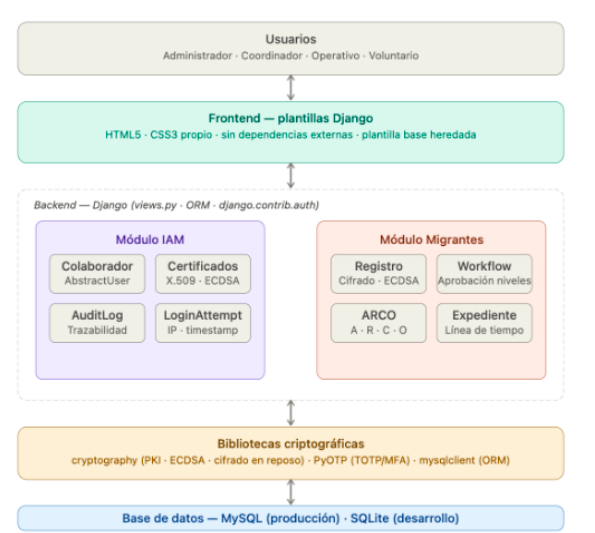
\includegraphics[width=0.82\textwidth]{diagram.png}
\caption{Diagrama de arquitectura del sistema de gestión de identidades y registro de migrantes de Casa
Monarca. Generado con Claude (Anthropic, 2026).}
\end{figure}

 
\subsection*{3.1 Backend}
 El backend del sistema se divide en dos módulos con modelos de datos independientes pero conectados. El módulo IAM (gestor de colaboradores) gestiona el ciclo de vida completo de un colaborador desde el alta con contraseña temporal hasta la baja o revocación, también registra cada intento de inicio de sesión, exitoso o no, incluyendo la dirección IP de origen, lo que permite al administrador anticipar posibles brechas de seguridad. El módulo de registro de migrantes implementa una cadena de auditoría criptográfica en la que cada firma generada encadena el hash de la firma anterior a través del campo \texttt{prev\_chain\_hash}. Esto resulta en que el historial de acciones sea verificable e inalterable, con esto logramos que la persona encargada de firmar no pueda decir que él no es el responsable de la acción. Adicionalmente, el modelo SignedFlowLog registra cualquier acción irreversible firmada con certificado X.509. Este es el único modelo del sistema que no permite editar ni eliminar, lo que garantiza que Casa Monarca pueda demostrar en todo momento la integridad de su cadena digital ante cualquier autoridad de ser necesario.


 
\subsection*{3.2 Frontend}
 La interfaz fue desarrollada con plantillas de Django en HTML5 y CSS propio, sin dependencias externas de frameworks, lo que garantiza que el sistema no dependa de recursos de terceros para su funcionamiento. Esto ayuda a que en caso de tener que emitir o revocar un certificado el administrador lo pueda hacer por sí mismo en el momento que lo desea. Cada pantalla depende del nivel del usuario autenticado, cada nivel tiene diferentes acciones disponibles, de modo que ningún colaborador puede visualizar ni ejecutar funciones fuera de su alcance. 

\begin{figure}[H]
\centering
\begin{minipage}{0.48\textwidth}
    \centering
    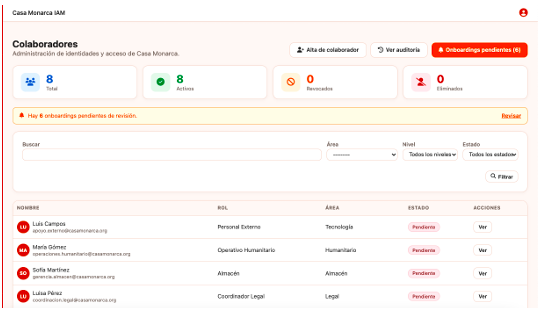
\includegraphics[height=0.18\textheight]{dashboard.png}
    \caption{Dashboard del gestor de colaboradores}
\end{minipage}\hfill
\begin{minipage}{0.48\textwidth}
    \centering
    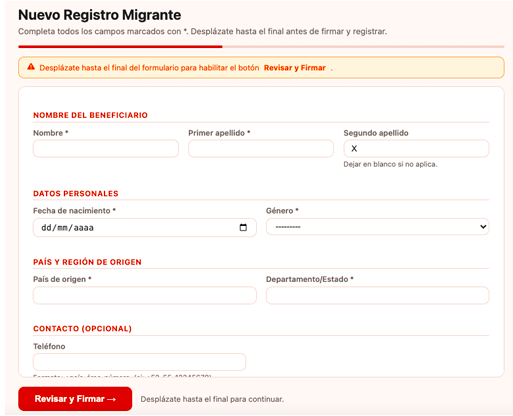
\includegraphics[height=0.18\textheight, trim=0 35 0 0, clip]{form.png}
    \caption{Formulario de registro de migrantes}
\end{minipage}
\end{figure}

 
%% ─── 5. IMPACTO DE NEGOCIO ─────────────────────────────────────────────────
\section*{4. Impacto de Negocio}
 
De acuerdo a proyecciones del equipo basadas en el flujo operativo estimado de Casa Monarca (35 colaboradores en promedio, 3 actualizaciones de la base por semana, 5 registros de migrantes semanales, aproximadamente 2 solicitudes ARCO por mes y procesos adicionales manuales), el sistema permite ahorrar un total de 189 horas/año. El ahorro financiero es un aproximado de \$700 USD por año al comparar el costo del sistema desarrollado frente a una solución comercial equivalente. Con la aplicación se mejora la productividad de los colaboradores, especialmente de aquellos que se involucran en el registro o ingreso de los colaboradores y migrantes  a Casa Monarca. Esto se debe a que se eficientizan los procesos y se vuelven digitales, bajando la cantidad de error humano al registrarse directamente en una base digital más que un proceso manual que después se tiene que registrar en línea. Esto permite que se realice todo en una misma interfaz, ahorrando tiempo y minimizando errores. Por otro lado, el sistema permite que el administrador emita certificados y lleve un rastreo de los movimientos de los colaboradores en el sistema, mejorando la seguridad de los procesos. La forma de medir la mejoría respecto a los procesos anteriores aunque tardada, es viable, y sería cronometrar el tiempo del proceso realizado manualmente y el proceso digitalizado por medio del sistema. Por otro lado, algo que no requiere comparación ni contabilidad, es el hecho de que se reduce el error humano.

\begin{table}[H]
\centering
\small
\begin{tabularx}{\textwidth}{Xr}
\toprule
\textbf{Concepto} & \textbf{Horas/año} \\
\midrule
Cambios frecuentes de colaboradores (3x semana $\times$ 52 sem) & \textasciitilde47 hrs \\
Registros de migrantes (5x semana $\times$ 52 sem)              & \textasciitilde69 hrs \\
Solicitudes ARCO (\textasciitilde2/mes)                          & \textasciitilde15 hrs \\
Revisiones periódicas de accesos (50 min/sem $\times$ 52)       & \textasciitilde43 hrs \\
Eliminación de re-capturas y errores de transcripción           & \textasciitilde15 hrs \\
\textbf{Total ahorrado}                                          & \textbf{\textasciitilde189 hrs} \\
\bottomrule
\end{tabularx}
\caption{Estimación de horas ahorradas al año con el sistema.}
\end{table}
 
\begin{table}[H]
\centering
\small
\begin{tabularx}{\textwidth}{Xr}
\toprule
\textbf{Concepto} & \textbf{Costo/año} \\
\midrule
Solución comercial             & \textasciitilde\$800 USD \\
Este sistema (hosting + dominio) & \textasciitilde\$100 USD \\
\textbf{Ahorro anual}          & \textbf{\textasciitilde\$700 USD} \\
\bottomrule
\end{tabularx}
\caption{Comparación de costos anuales entre el sistema desarrollado y una solución comercial equivalente.}
\end{table}

%% ─── 6. LECCIONES Y HALLAZGOS ──────────────────────────────────────────────
\section*{5. Lecciones y Hallazgos}
 
Con Django, se identificó que era buena opción desde un inicio, ya que cuenta con elementos de protección integrados que son cruciales para la protección de las bases de datos manipuladas por los colaboradores de Casa Monarca. Entre esos elementos, se encuentra seguridad contra:

\begin{itemize}[leftmargin=*]
    \item \textit{Cross-Site Scripting} (XSS): ataque en el que un actor malicioso inyecta código JavaScript en una página web para que se ejecute en el navegador de otro usuario. Esto se hace con el fin de robar sesiones o datos sensibles.
    \item \textit{Cross-Site Request Forgery} (CSRF): ataque en el que se engaña al navegador de un usuario autenticado para que envíe una solicitud no autorizada a su nombre. Esto hace que se realicen acciones sin consentimiento.
    \item \textit{SQL Injection}: ataque en el que se insertan instrucciones SQL maliciosas en un campo de entrada para manipular o extraer datos directamente de la base de datos.
    \item \textit{Clickjacking}: ataque en el que se superpone una página invisible sobre una legítima para que el usuario haga clic en elementos ocultos sin saberlo, ejecutando acciones no deseadas.
\end{itemize}

Además, se descubrió que usar el framework de Django es sostenible a largo plazo. Esto se debe a que su documentación es extensa y es comúnmente utilizada. Al ser código abierto, es gratuito y por lo tanto ideal para una organización como Casa Monarca. 
Dentro de los hallazgos del proyecto, se identificó que Keycloak, aunque era una herramienta útil que podía simplificar el desarrollo del proyecto IAM (gestor de identidades y accesos), se concluyó en que al no ser compatible con Hostgator, y añadir costos por infraestructura (aunque no por el propio uso de Keycloak), no era una opción a considerar en este caso en específico. 
Logramos identificar también que un sistema que parece ser un simple gestor de identidades, involucra aspectos como el rastreo de actividad por medio de la auditoría, la emisión de certificados personales, y asignación de nivel y área, así como los permisos dependiendo de lo mismo. Aunque un gestor de identidades puede ser utilizado en múltiples entornos, compañías y/o organizaciones, este se puede personalizar, y son esos detalles lo que diferencian a un sistema de otro. Además, se implementó el gestor de registros que es esencial para mantener los datos de los migrantes seguros.
La elección de ECDSA sobre RSA demostró ser acertada en la práctica, se logra ofrecer el mismo nivel de seguridad de 128 bits con claves más pequeñas (256 bits contra 3,072 bits de RSA). Los archivos \texttt{.cert} y \texttt{.key} resultaron suficientemente ligeros y sencillos para que personal no técnico los cargue manualmente en cada inicio de sesión. 
La interfaz logró la usabilidad para usuarios sin perfil técnico, la cuál era una de nuestras metas. Las pantallas son sencilas y logran guíar al colaborador paso a paso. Hay mensajes de error que indican con precisión qué salió mal y cómo se pueden corregir. Las acciones irreversibles como confirmar un registro, ejecutar una cancelación ARCO o revocar un certificado requieren confirmación explícita antes de ejecutarse, reduciendo los errores humanos.Todo esto se traduce en una capacitación más corta y rápida por parte del equipo de Casa Monarca.

 
%% ─── 7. ESTADO ACTUAL Y PRÓXIMOS PASOS ────────────────────────────────────
\section*{6. Estado Actual y Próximos Pasos}
 
El sistema se encuentra actualmente completo en sus dos módulos: gestor de identidades y registro de migrantes. La solución está lista para su despliegue en el servidor de Casa Monarca. Los módulos IAM y de registro de migrantes fueron validados en un entorno de desarrollo local con base de datos SQLite, y la configuración para producción con MySQL se encuentra preparada. El siguiente paso es la instalación en el servidor de Casa Monarca, que al ser compatible con el stack tecnológico elegido desde el inicio del proyecto, no representa un costo adicional para la organización ni requiere cambios de infraestructura.
En los próximos pasos se encuentra la capacitación del personal, comenzando por el administrador, quien será el responsable del ciclo de vida de los colaboradores y de la emisión de certificados. Para este proceso se cuenta con un manual de usuario que cubre los flujos principales del sistema, el manual va dirigido a todos los niveles, contando con una sección por nivel. También, se recomienda desarrollar dos mejoras: 
\begin{itemize}[leftmargin=*]
    \item Un sistema de notificaciones automáticas por correo que alerte al administrador ante cualquier cambio irreversible, como una revocación de certificado o una cancelación ARCO.
    \item Un mecanismo de respaldo automático de la base de datos.
\end{itemize}

 
%% ─── 8. REFERENCIAS ────────────────────────────────────────────────────────
\section*{7. Referencias}
 
\begin{itemize}[leftmargin=*, label={}]
 
\item Anthropic. (2026). \textit{Claude} (Claude Sonnet 4.6) [Modelo de lenguaje de gran escala]. Recuperado de \url{https://www.anthropic.com} (empleado como asistente de generación del diagrama de arquitectura).

\item Boeyen, S., Santesson, S., Polk, T., Housley, R., Farrell, S., \& Cooper, D. (2008). \textit{Internet X.509 Public Key Infrastructure Certificate and Certificate Revocation List (CRL) Profile} (RFC 5280). RFC Editor. Disponible en: \url{https://datatracker.ietf.org/doc/rfc5280/}
 
\item Cámara de Diputados del H. Congreso de la Unión. (2010). \textit{Ley Federal de Protección de Datos Personales en Posesión de Particulares}. Diario Oficial de la Federación. Disponible en: \url{https://www.diputados.gob.mx/LeyesBiblio/pdf/LFPDPPP.pdf}
 
\item Django Software Foundation. (2026). \textit{Django documentation}. Disponible en: \url{https://www.djangoproject.com/}
 
\item Keycloak Project. (2026). \textit{Keycloak documentation}. Disponible en: \url{https://www.keycloak.org/}
 
\item National Institute of Standards and Technology. (2023). \textit{FIPS 186-5: Digital Signature Standard (DSS)}. Disponible en: \url{https://nvlpubs.nist.gov/nistpubs/FIPS/NIST.FIPS.186-5.pdf}
 
\item Smallstep Labs. (2026). \textit{step-ca documentation}. Disponible en: \url{https://smallstep.com/docs/step-ca/}
 
\item Zamora G., J. (2018). \textit{Migración sudamericana en México} [Tesis]. El Colegio de la Frontera Norte. Disponible en: \url{https://posgrado.colef.mx/tesis/uec2017329/}
 
\end{itemize}
 
\end{document}